Throughout this section the theory of the key ideas of the experimental setup is explained. This section will enlighten the basics of neural networks, the image specific convolutional neural network, transfer learning which were used to fine-tune the top layers of the CNNs proposed in this study, ideas in contrastive learning that could prove to be a huge improvement in reaching the objective of the problem definition, and the similarity measurement which is used to describe how well the models perform. \\
\textbf{Jump to sections} \hyperref[sec:Neural]{Neural Networks}, \hyperref[sec:Convolutional]{Convolutional NN}, \hyperref[sec:Transfer]{Transfer Learning}, \hyperref[sec:contrastive]{Contrastive Learning} and \hyperref[sec:Similarity]{Measuring of Similarity}.
\subsection{Neural Networks}\label{sec:Neural}
Before progressing through the report the basics of neural networks should be understood.
Neural networks comes from the idea of being able to teach a computer how to process an input, fundamentally similar to a brain, but without doing any programming (i.e. \texttt{If..else statements}).
The human brain consists of 100 billions neurones, the neurones are what make the humans capable of interpreting signals from the outside world. The neurones are able to adapt themselves to react different if a certain scenario happens. The neural networks also uses neurones to interpreting inputs:
\begin{figure}[H]
    \centering
    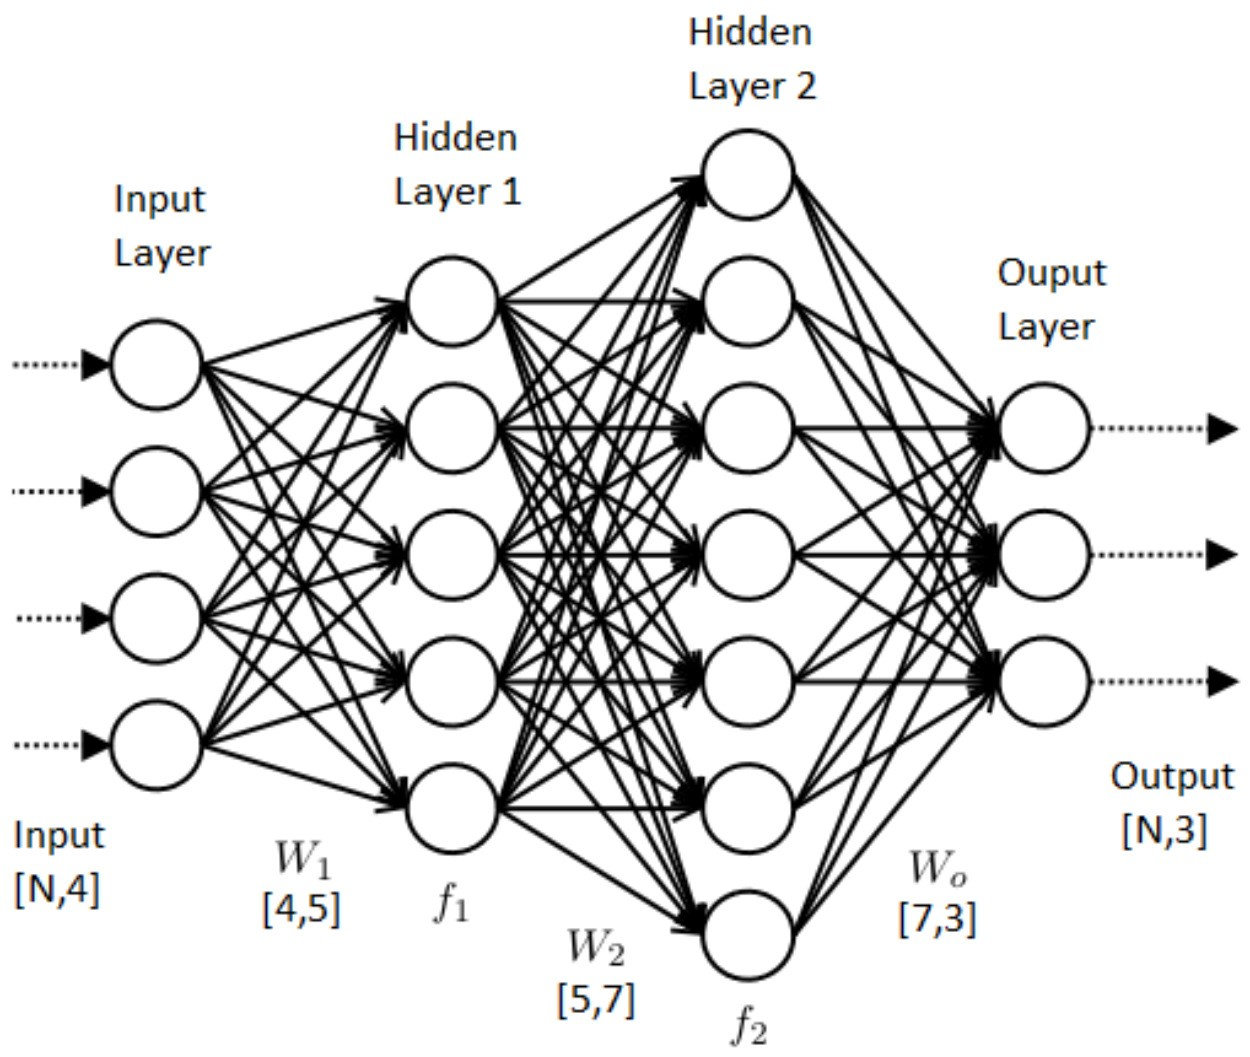
\includegraphics[width = 0.6\textwidth]{pictures/random/simpleneuralnetwork}
    \caption{A simple neural network consisting of an input layer, two hidden layers, and an output layer}
    \label{ref:Loss}
\end{figure}
The figure, \autoref{ref:Loss}, show a simple neural network, that consists of an input layer, two hidden layers and an output layer. Each layer consist of a various numbers of neurones, each neurone in a layer is connected to all the neurones in the next layer by weights, the weights define what information the neurone should forward to the next layer of neurones. Neural networks often involve adaptiveness of weights, which means that the neural network will be able to learn new ways of interpreting inputs. The weights are adapted through a learning algorithm, and a target value. The target value is what the neurone should accomplish, and the learning algorithm is how the weights should the updated, if the target is not achieved. All subsequent inputs will be processed by using the updated weights.
\newpage
\epigraph{All models are wrong, but some are useful.}{George E. P. Box}
\subsection{Convolutional Networks}\label{sec:Convolutional}
The convolutional neural network\autocite{dumoulin2018guide}, denoted CNN, is a specific construction of neural networks, which has proven to be very useful when working with images. Convolutional networks uses convolutional filters between each layers. Convolutional networks have the advantage of being able to interpret the relationship between integers for all axes on each layer. This is what makes them suitable for understanding the relation between pixels in images. On the lowest levels of the convolutional network, the CNN will learn how to recognise edges and simple shapes. The higher the level of layers the more abstract and complicated the shapes. Below, \autoref{ref:convolutionarchitecture}, it is shown how the convolutional filters work on each layer. Each layer of the network changes dimensions, so new convolutions can be applied and more complex shapes can be identified.
\begin{figure}[H]
    \centering
    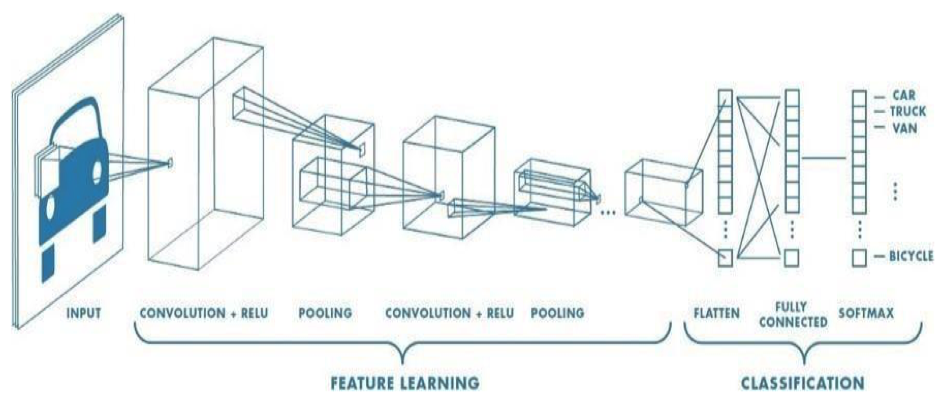
\includegraphics[width = \textwidth]{pictures/random/convolutionarchitecture}
    \caption{Architecture of a Convolutional Neural Network.\\
    Image from: https://arxiv.org/pdf/2101.00793.pdf page. 8}
    \label{ref:convolutionarchitecture}
\end{figure}
\hyperref[ref:MNIST]{Below} are shown different convolutions applied to one of the images in the MNIST dataset\footnote{http://yann.lecun.com/exdb/mnist/}, picturing the number 7. From these representations the CNN is able to learn different ways of interpreting this picture, the model is concatenating the interpretations from the convolution layers in the pooling layers.
\begin{figure}[H]
    \centering
    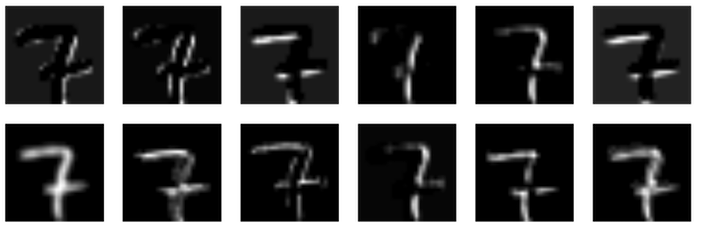
\includegraphics[width = 0.8\textwidth]{pictures/random/mnist}
    \caption{Different convolutions applied to the mnist dataset.\\
    Image from: https://sempwn.github.io/blog/2017/04/06/conv\_net\_intro}
    \label{ref:MNIST}
\end{figure}
The above case is simple compared to the object of this study, which is to measure similarities in different rooms, however the procedure is the same. Identifying objects in rooms and map the objects to specific labels, for example: a sink for kitchen, a bed for bedroom or couch for living room. These are the very obvious cases, some of the images of kitchens don't include sinks, and then hopefully the model has learned other representations which evaluates to kitchen. When training a network from the ground and up, a lot of data is required, and often data is very expensive to acquire. To accommodate the need for large and hence expensive data sets, other methods such as transfer learning can be applied that are less dependent on large data sets.
